\section{Rappels réseaux}

\begin{frame}[fragile]
  \frametitle{Rappels réseaux}
\begin{center}
	\Huge{\bf\color{blue}Rappels réseaux}
\end{center}
\begin{flushright}
  \item Préalables
  \item Modèle OSI
  \item Modèle TCP/ IP
  \item Ethernet
\end{flushright}
\end{frame}

\begin{frame}[fragile]
  \frametitle{Rappels réseaux}
{\bf\Large Préalable}

Afin de modéliser le fonctionnement des réseaux, la complexité est décomposée en
\textbf{couches}; chaque couche repose sur la couche inférieure afin d'offrir
des services à la couche supérieure
\begin{itemize}
	\item Modèle OSI
	\item Modèle TCP / IP
	\item Ethernet
\end{itemize}
\end{frame}


\section{Rappels réseaux - Modèle OSI}

\begin{frame}[fragile]
  \frametitle{Rappels réseaux - Modèle OSI}
Le \textbf{modèle OSI} propose un découpage en 7 couches. 
À ces couches sont associés des protocoles que nous n'étudions pas.

\begin{center}
	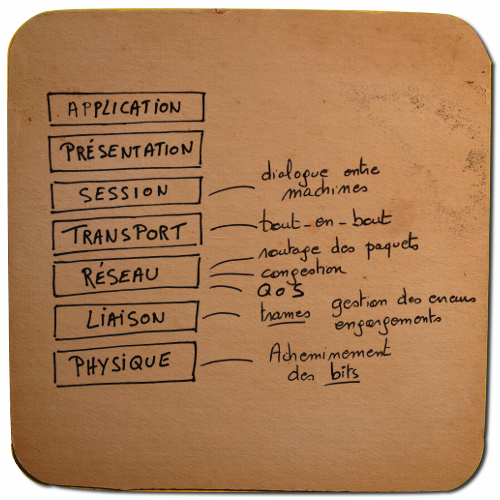
\includegraphics[width=.55\linewidth]{img/modele-osi-500x500.png}
\end{center}
\end{frame}

\begin{frame}[fragile]
  \frametitle{Rappels réseaux - Modèle OSI}
\begin{itemize}
	\item Couche physique (\textit{physical layer})
	\begin{itemize}
		\item Transmission des bits sur le support
		\item Gestion des différents supports; fibre optique, cuivre, onde radio, courant porteur, ...
	\end{itemize}
	\item Couche liaison de données (\textit{data link layer})
	\begin{itemize}
		\item Montrer à la couche \textit{network}, une transmission sans
		erreurs non détectées
		\item Transmet des \textbf{trames} de données
		\item Doit gérer les différences de vitesse entre l'émetteur et le récepteur (engorgement)
	\end{itemize}
	\item Couche réseau (\textit{network layer})
	\begin{itemize}
		\item Transmet de \textbf{paquets} de données
		\item Détermine comment les paquets sont routés d'un point à un autre
		\item Gestion de la congestion et de la qualité de service
	\end{itemize}
\end{itemize}
\end{frame}

\begin{frame}[fragile]
  \frametitle{Rappels réseaux - Modèle OSI}
\begin{itemize}
	\item Couche transport 	(\textit{transport layer})
	\begin{itemize}
		\item Accepte des données de la couche supérieure et les transmet
		\item Veille à la transmission de bout en bout
		\item Autorise différents types de services; point-à-point sans erreur, diffusion à plusieurs destinataires, ...
	\end{itemize}
	\item Couche session (\textit{session layer}
	\begin{itemize}
		\item Permet l'établissement d'une session (dialogue, synchronisation, ...)
	\end{itemize}
	\item Couche présentation (\textit{presentation layer})
	\begin{itemize}
		\item Permet une certaine abstraction des données transmises
	\end{itemize}
	\item Couche application (\textit{application layer})
	\begin{itemize}
		\item Définit les différents protocoles; http, smtp, ftp, ...
	\end{itemize}
\end{itemize}
\end{frame}

\begin{frame}[fragile]
  \frametitle{Rappels réseaux - Modèle OSI}
\begin{center}
	{\Large Nous nous concentrerons sur les couches \\ 
	\textit{physical, data link} et \textit{network}}
\end{center}
\end{frame}


\section{Rappels réseaux - Modède TCP / IP}

\begin{frame}[fragile]
  \frametitle{Rappels réseaux - Modède TCP / IP}
Le \textbf{modèle TCP / IP} propose également un découpage en couches. On s'intéresse particulièrement aux protocoles associés au modèle.

\begin{center}
	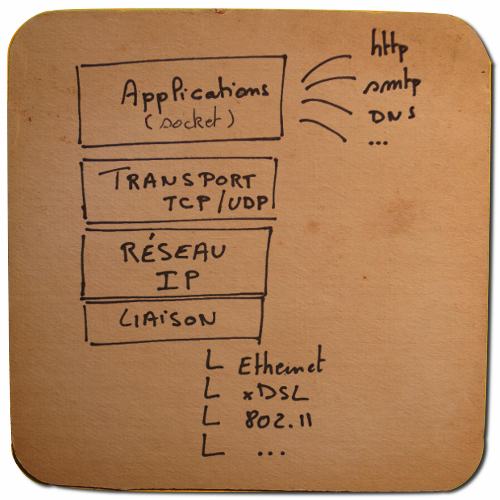
\includegraphics[width=.55\linewidth]{img/modele-tcpip-500x500.png}
\end{center}
\end{frame}

\begin{frame}[fragile]
  \frametitle{Rappels réseaux - Modède TCP / IP}
\begin{itemize}
	\item Interface de liaison
	\begin{itemize}
		\item Permet de faire un lien entre le support physique et l'adresse IP de la machine
		\item Les protocoles associés, ethernet, SONET, xDSL, 802.x
	\end{itemize}
	\item Couche internet (\textit{internet layer})
	\begin{itemize}
		\item Permet l'introduction de paquets sur le réseau ...
		\item ... ces paquets seront acheminés vers l'hôte de destination (même sur un autre réseau)
		\item \textbf{Les} protocoles associés sont \textbf{IP} et ICMP
	\end{itemize}
	\item Couche transport (\textit{transport layer})
	\begin{itemize}
		\item Permet à deux hôtes de communiquer
		\item \textbf{Les} protocoles associés sont \textbf{TCP} et \textbf{UDP}
		\begin{itemize}
			\item TCP, protocole fiable avec connexion assure le contrôle de flux
			\item UDP, protocole non fiable sans connexion
		\end{itemize}
	\end{itemize}
	\item Les applications
\end{itemize}
\end{frame}


\section{Rappels réseaux - Ethernet}

\begin{frame}[fragile]
  \frametitle{Rappels réseaux - Ethernet}
Deux normes proches / confondues; \textbf{802.3} et \textbf{Ethernet}

Distinguer
\begin{itemize}
	\item Ethernet classique
	\begin{itemize}
		\item Débit 3-10 Mbit/s
	\end{itemize}
	\item Ethernet commuté
	\begin{itemize}
		\item Utilisation de commutateurs (\textit{switch})
		\item Débit 100 Mbit/s pour «Fast Ethernet»
		\item Débit 1 Gbit/s pour «Gigabit Ethernet»
		\item Débit 10 Gbit/s
	\end{itemize}
\end{itemize}
\end{frame}

\begin{frame}[fragile]
  \frametitle{Rappels réseaux - Ethernet}
{\large\bf Couche physique}
\begin{itemize}
	\item Jadis, cable coaxial
	\item Paire torsadée
\end{itemize}

{\large\bf Sous couche d'accès au réseau (\textit{Media Access Control})}
\begin{itemize}
	\item Format de la trame Ethernet \\
	\begin{center}
		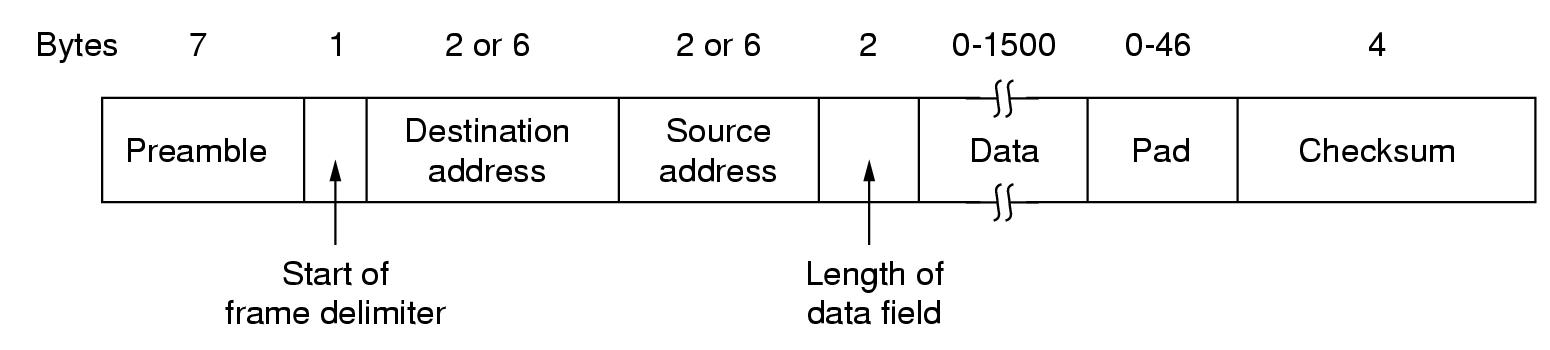
\includegraphics[width=.90\linewidth]{img/4-21.jpg} \\
		{\scriptsize Format de trame IEEE 802.3 (presque Ethernet) - Image de
		[Tanenbaum]}
	\end{center}
\end{itemize}
\end{frame}

\begin{frame}[fragile]
  \frametitle{Rappels réseaux - Ethernet}
{\large\bf Format de la trame Ethernet}
\begin{itemize}
	\item Préambule
	\begin{itemize}
		\item 8 fois 10101010b pour Ethernet
		\item 7 fois 10101010b pour 802.3, suivi du « Start of Frame » 10101011b
		\item Le codage Manchester de ces 8 \textit{bytes} produit un signal
		rectangulaire (10MHz pendant 6,4µs) permettant la synchronisation de l'horloge
	\end{itemize}
	\item Format des adresses
	\begin{itemize}
		\item Les champs adresses font 6 bytes
		\item Appelée « adresse MAC »; 3 premiers bytes pour le fabricant, 3 derniers pour la carte
		\item Différenciation
		\begin{itemize}
			\item Premier bit 0 pour adresse ordinaire
			\item Premier bit 1 pour adresse de groupe (diffusion \textit{multicast})
			\item Si tous les bits sont à 1 \textit{broadcast}
		\end{itemize}
	\end{itemize}
\end{itemize}
\end{frame}

\begin{frame}[fragile]
  \frametitle{Rappels réseaux - Ethernet}
{\large\bf Format de la trame Ethernet (suite)}
\begin{itemize}
	\item Type de la trame (Ethernet) ou longueur (802.3)
	\begin{itemize}
		\item Par exemple; 0x800 pour dire que la trame contient paquet IPv4
		\item Si la valeur est inférieure à 0x600, elle représente la longueur sinon, c'est le type
	\end{itemize}
	\item Données
	\begin{itemize}
		\item Maximum 1500 bytes
		\item Minimum 46 bytes (pour que la trame fasse minimum 64 bytes)
	\end{itemize}
\end{itemize}
\end{frame}

\begin{frame}[fragile]
  \frametitle{Rappels réseaux - Ethernet}
{\large\bf Format de la trame Ethernet (suite)}
\begin{itemize}
	\item Détection de collisions
	\begin{itemize}
		\item Le signal de brouillage peut mettre $2\tau$ pour revenir à l'émetteur 
		\item Dans LAN 10Mbit/s, $2\tau$ est proche de $50\mu s$  la trame
		doit donc avoir une longueur de 500 bits. On arrondi à 512 bits = 64
		bytes
	\end{itemize}
\end{itemize}
\begin{center}
	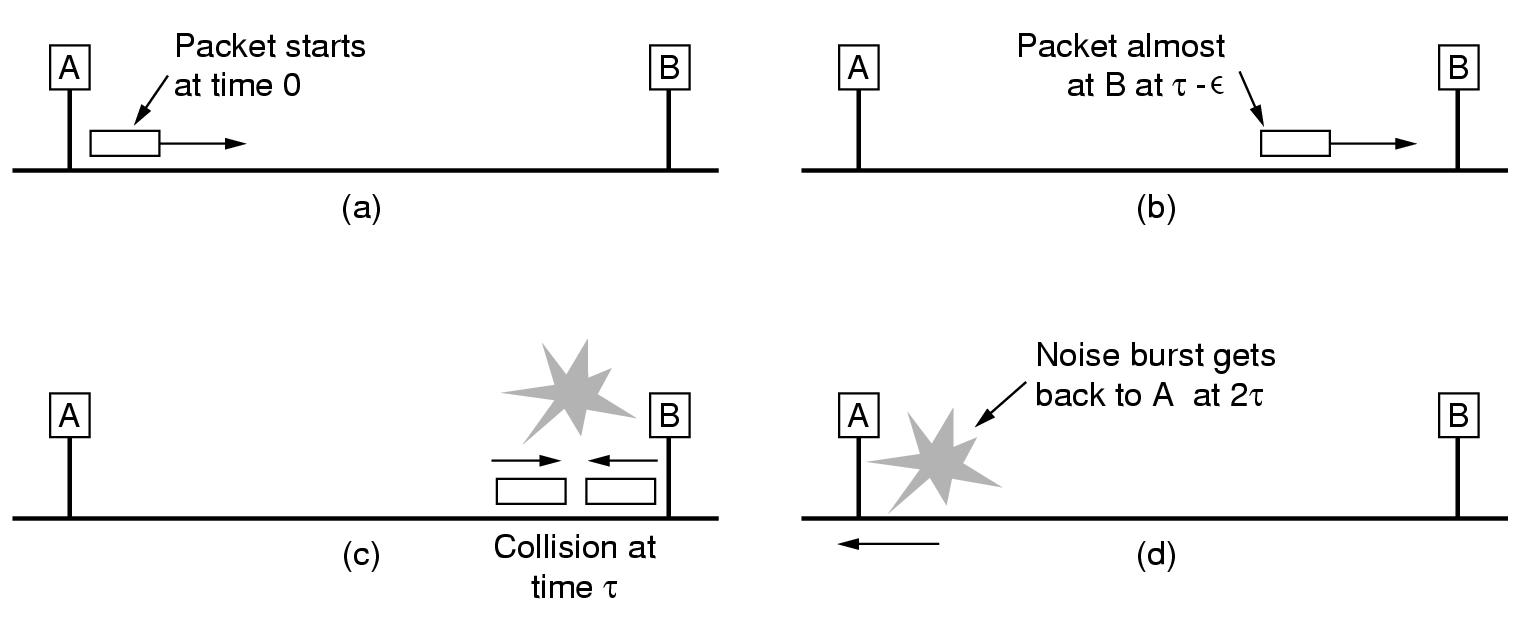
\includegraphics[width=.80\linewidth]{img/4-22.jpg} \\
	{\scriptsize Détection de colision - Image de [Tanenbaum]}
\end{center}
\end{frame}

\begin{frame}[fragile]
  \frametitle{Rappels réseaux - Ethernet}
{\large\bf Format de la trame Ethernet (suite)}
\begin{itemize}
	\item Total de contrôle (\textit{checksum})
	\begin{itemize}
		\item Si erreur, la trame est supprimée
		\item Valeur CRC de 32 bits
	\end{itemize}
\end{itemize}
\end{frame}


\begin{frame}[fragile]
  \frametitle{Rappels réseaux - Ethernet}
{\large\bf Exercice}
Observer le format d'une trame éthernet 
\begin{itemize}
	\item Utilisation de Wireshark
	\item Faire passer une trame et repérer les \textit{MAC address}
	\item Constater / vérifier que le mode promicuous ne fonctionne pas avec un switch
	\item Liens / références / aide
	\begin{itemize}
		\item Wireshark \url{http://www.wireshark.org}
		\item\url{http://wiki.wireshark.org/Ethernet}
	\end{itemize}
\end{itemize}
\end{frame}


